%%%%%%%%%%%%%%%%%%%%%%%%%%%%%%%%%%%%%%%%%%%%%%%%%%%%%%%%%%%%%%%%%%%%%%%%%%%%%%%%
\section{Improving PDF Fits with lattice QCD calculations}
\label{sec:projections}
%%%%%%%%%%%%%%%%%%%%%%%%%%%%%%%%%%%%%%%%%%%%%%%%%%%%%%%%%%%%%%%%%%%%%%%%%%%%%%%%

In this section we aim to provide an initial estimate of the potential  impact of
present and future lattice-QCD calculations
in global unpolarised and polarised PDF fits.
%
This study will be carried out by means of the publicly available
Bayesian reweighting
method~\cite{Ball:2011gg,Ball:2010gb} applied to the
NNPDF3.1 NNLO an NNPDFpol1.1 sets.
%
We emphasize however that the qualitative results that are found here
should apply as well to other PDF sets, for example
if the Hessian profiling method~\cite{Camarda:2015zba} was used to assess the
impact of the same lattice calculations into a Hessian sets.
%
Both approximate methods allow to quantify the impact of new measurements
(or of future measurements, if pseudo-data is used) on a PDF set without
having to redo the global analysis again.

For simplicity, we will restrict  ourselves here to study the
impact of a subset of the moments that can be
evaluated using lattice QCD.
%
In particular,
we will focus on those that can be currently calculated
with the smallest uncertainties, as discussed in
Sect.~\ref{sec:benchmarking}.
%
We do not consider other of the moments discussed in
Sect.~\ref{Sec:IntroLQCD} and Appendix~\ref{sec:LQCDtables}
since these are typically affected by larger systematic uncertainties.
%
Likewise, we won't consider  in this exercise pseudo-data based on $x$-space
lattice QCD calculations, such as those from the quasi-PDF approach,
since as shown in Sect.~\ref{sec:xdependence}, despite the rapid
recent progress, existing calculations are still far to the
phenomenological PDFs.
%
We leave for future work quantifying the impact of  $x$-space
lattice QCD calculations of PDFs in the global analysis.

Taking into account
these considerations, we will consider in this analysis the following
moments.
%
For the unpolarized case, we will use
\be
  \la x\ra_{u^+}\, , \quad
\la x\ra_{d^+}\, , \quad
\la x\ra_{s^+}\, , \quad
\la x\ra_{g}\, , \quad {\rm and} \quad
\la x\ra_{u^+-d^+} \, ,
\ee
while for the polarized side, we will include instead
the following five moments:
\be
\la 1\ra_{\Delta u^+}\, , \quad
\la 1\ra_{\Delta d^+}\, , \quad
\la 1\ra_{\Delta s^+}\, , \quad
\la x\ra_{\Delta u^--\Delta d^-}\, , \quad {\rm and} \quad
\la 1\ra_{\Delta u^+ - \Delta d^+} \, .
\ee
Recall that Appendix~\ref{app:notation} contains the
explicit definitions and conventions used for these moments.
%
Therefore, we see that for the unpolarized case we include
the second moments (momentum fractions) of $q^+$ (with $q=u,d,s$),
of the gluon, and of the isoscalar combination $u^+-d^+$.
%
In the polarized case instead, we include the first moments (which
contribute to the proton spin content) of $\Delta q^+$ (with $q=u,d,s$)
and of the isoscalar combination $\Delta u^+-\Delta d^+$, as well as
the second moment of $\Delta u^- - \Delta d^-$.

Moreover, we will consider in the present exercise three
different scenarios, which we denote
as Scenario A, B, and C, respectively, for the total systematic
uncertainty than we associate to lattice
QCD calculations of PDF moments.
%
In Table~\ref{tab:scenarios} we summarize the
values assumed of total uncertainty
    in the lattice QCD calculation, $\delta_L$, for each
    of the various unpolarized and polarized PDF moments that enter
    this analysis.
    %
    First of all, scenario A assumes that the uncertainties $\delta_L$
    are on the ball-park of the current ones, taking as
    representative values  those from the
    state-of-the-art lattice QCD calculations
    selected for the benchmarking exercise of Sect.~\ref{sec:benchmarking},
    and summarized in Tables~\ref{tab:BMunp} and~\ref{tab:BMpol}.
    %
    Then scenarios B and C represent two possible optimistic scenarios for the
    future improvement of these systematic uncertainties.
    %
    We emphasize that, while we try to be reasonably
    realistic, we do not aim here to classify a given scenario
    as more or less feasible within a given time scale:
    the results here are merely illustrative of the possible
    constraining power of PDF calculations in the context
    of a global PDF analysis.

%%%%%%%%%%%%%%%%%%%%%%%%%%%%%%%%%%%%%%%
\begin{table}[t]
  \centering
  \renewcommand{\arraystretch}{1.3} 
  \begin{tabular}{c||ccccc}
    \hline
    Scenario &  \multicolumn{5}{c}{$\delta_L$ for unpolarized moments}   \\
&    $\la x\ra_{u^+}$  &   $\la x\ra_{d^+}$   &  $\la x\ra_{s^+}$  &
$\la x\ra_{g}$  &   $\la x\ra_{u^+-d^+}$  \\
    \hline
    Current  & $\sim 16\%$  &  $\sim 30\%$
    & $\sim 45\%$  & $\sim 13\%$  &  $\sim 60\%$ \\
    A   & 20\%  & 30\% &  50\% &  15\% &  60\% \\
 B   & 10\%  & 15\% &  25\% &  7\% &  30\%  \\
  C   & 5\%  & 7\% &  12\% &  3\% &  15\%  \\
    \hline
  \end{tabular}\vspace{0.7cm}
   \begin{tabular}{c||ccccc}
    \hline
    Scenario   &
    \multicolumn{5}{c}{$\delta_L$ for polarized moments} \\ 
& $\la 1\ra_{\Delta u^+}$  & $\la 1\ra_{\Delta d^+}$  & $\la 1\ra_{\Delta s^+}$
&  $\la x\ra_{\Delta u^--\Delta d^-}$  &  $\la 1\ra_{\Delta u^+ - \Delta d^+}$\\
    \hline
    Current  &
    $\sim 3\%$  & $\sim 5\%$ & $\sim 70\%$ & $\sim 65\%$ & $\sim 3\%$ \\
    \hline
    A   & 
    5\% &    10\%  &   100\% &    70\%  &    5\% \\
 B   &
 3\% &    5\%  &   50\% &    30\%  &    3\% \\
  C   & 1\% &    2\%  &   20\% &    15\%  &    1\% \\
    \hline
  \end{tabular}
   \caption{\small The three scenarios assumed here
     for the total percentage
     systematic uncertainty
    in future lattice QCD calculation $\delta_L$ for each
    of the unpolarized (upper) and polarized (lower table) PDF
    moments that are included
    in the present reweighting analysis.
    %
    In addition, the first line indicates the current systematic
    uncertainties of the state-of-the-art lattice QCD calculations
    selected for the benchmarking exercise of Sect.~\ref{sec:benchmarking},
    and summarized in Tables~\ref{tab:BMunp} and~\ref{tab:BMpol}
    for the unpolarized and polarized cases, respectively.
    %
    See text for more details.
\label{tab:scenarios}
  }
\end{table}
%%%%%%%%%%%%%%%%%%%%%%%%%%%%%%%%%%%%%%%

The procedure followed to quantify the impact of future
lattice QCD calculations of these
PDF moments is the same in the case of the unpolarized
and polarized global analyses.
We briefly describe it here:
\begin{itemize}
\item First of all, we generate pseudo-data for the lattice QCD calculation
  of the PDF moments:$\la x\ra_{u^+}$,
$\la x\ra_{d^+}$,
$\la x\ra_{s^+}$,
$\la x\ra_{g}$, and
  $\la x\ra_{u^+-d^+}$ for the unpolarized case, and
  $\la 1\ra_{\Delta u^+}$,
$\la 1\ra_{\Delta d^+}$,
$\la 1\ra_{\Delta s^+}$,
$\la x\ra_{\Delta u^--\Delta d^-}$, and
  $\la 1\ra_{\Delta u^+ - \Delta d^+}$ for the polarized case.
\item This pseudo-data is constructed by taking the central values from
  the corresponding NNPDF fits (NNPDF3.1NNLO for the unpolarized case, and NNPDFpol1.1NLO
  for the polarized one). That is, we assume for simplicity that the central value
  of such future lattice calculations would coincide with those of the global fit.
\item The percentage uncertainty in the pseudo data is taken to be that indicated in
  Table~\ref{tab:scenarios} for each of the three scenarios.
\item Using these central values and total uncertainties of the pseudo-data, we compute
  weights for each of the $N_{\rm rep}=1000$~(100) replicas of the input PDF set
  in the unpolarized (polarized) case.
  %
  These weights $w_k$ are a measure of the agreement of the individual replicas with the new pseudo-data.
  For instance replicas which lead to moments far from the pseudo-data (within uncertainties) will
  heave associated a very large weight.
\item These weights can be use to now recompute the PDFs and their moments, and emulate the
  impact that adding these pseudo-data points in a complete PDF fit would have (provided
  the effective number of replicas is not too small, see below).
  \end{itemize}

In Table~\ref{tab:neff} we indicate the effective number of replicas
    $N_{\rm eff}$ remaining when the pseudo-data
    on the PDF moments is included in the global
    fit according to the three scenarios outlined
    in Table~\ref{tab:scenarios}.
    %
    For completeness, we also indicate here the original number
    of replicas $N_{\rm rep}$ for the original
    PDF sets, NNPDF3.1 NNLO and NNPDFpol1.1 respectively.
    %
    As we can see, there is a marked decrease of $N_{\rm rep}$
    for the three scenarios, indicating that adding the
    PDF moments leads to non-trivial constraints on the global
    fit.
    %
    For instance, in the most optimistic scenario,
    Scenario A, the effective number of replicas is around five (three)
 smaller than the starting number of replicas.

%%%%%%%%%%%%%%%%%%%%%%%%%%%%%%%%%%%%%%%%%%%%%%
\begin{table}[t]
  \centering
  \begin{tabular}{c|c|c}
    \hline
    &  NNPDF3.1 NNLO  &  NNPDFpol1.1 \\
    \hline
    \hline
    $N_{\rm rep}$   &   1000 &  100   \\
    \hline
    Scenario A: $N_{\rm eff}$    &   211  &  35   \\
    Scenario B: $N_{\rm eff}$    &   670   &   54  \\
    Scenario C: $N_{\rm eff}$    &   680  &   58  \\
    \hline
  \end{tabular}
  \caption{\small The effective number of replicas
    $N_{\rm eff}$ remaining when the pseudo-data
    on the PDF moments is included in the global
    fit according to the scenarios outlined
    in Table~\ref{tab:scenarios}.
    %
    For completeness, we also indicate the original number
    of replicas $N_{\rm rep}$ for the original
    PDF sets, NNPDF3.1 NNLO and NNPDFpol1.1 respectively.
    \label{tab:neff}
  }
\end{table}
%%%%%%%%%%%%%%%%%%%%%%%%%%%%%%%%%%%%%%%%%%%%%%

\subsection{Impact on unpolarized global fits}
%
We start by discussing the results of applying the reweighting procedure
outlined above to a representative unpolarized
global fit, in this case the NNPDF3.1 NNLO analysis.

To begin with, in Table~\ref{tab:unpolmomentsrw} we summarize
the values of the unpolarized PDF moments
  used as pseudo-data, as well as the corresponding results
  after the reweighting has been performed for the
three scenarios summarized in 
in Table~\ref{tab:scenarios}.
%
As we can observe from this comparison, ....

%%%%%%%%%%%%%%%%%%%%%%%%%%%%%%%%%%%%%%%%%%%%%%%%%%%%%%%%
\begin{table}[h]
\centering
\begin{tabular}{c|c|c|c|c}
  \hline &  before RW  & RW Scen A  &  RW Scen B  & RW Scen C  \\
  \hline
  \hline
  $\la x\ra_{u^+}$     &  $0.348 \pm  0.004$   &  $ 0.349 \pm 0.002$     &     &   \\
  $\la x\ra_{d^+}$     &  $0.196\pm  0.004$   & $0.196 \pm0.002$      &     &   \\
  $\la x\ra_{s^+}$     & $0.0393 \pm 0.0036$   &  $0.0393\pm 0.0006$   &     &   \\
  $\la x\ra_{g}$      &   $0.4097\pm 0.0042$  &  $0.4097 \pm 0.0029$    &     &   \\
  $\la x\ra_{u^+-d^+}$  &  $0.1522 \pm 0.0033$  &  $0.1521 \pm 0.0019$   &     &   \\
  \hline
\end{tabular}
\caption{\small Values of the unpolarized PDF moments
  used as pseudo-data, as well as the corresponding results
  after the reweighting has been performed for the
three scenarios summarized in 
in Table~\ref{tab:scenarios}.
%
The PDF uncertainties quoted correspond in all cases to 68\%
CL intervals.
\label{tab:unpolmomentsrw}
}
\end{table}
%%%%%%%%%%%%%%%%%%%%%%%%%%%%%%%%%%%%%%%%%%%%%%%%%%%%%%%%

In Fig.~\ref{fig:impactUnpol} we show
percentage PDF uncertainty in NNPDF3.1 NNLO
  for the gluon and the $u^+$, $d^+$ and $s^+$ quark PDFs,
  compared to the results of including the five lattice
  QCD moments as pseudo-data points in the fit using the three
  different scenarios in  Table~\ref{tab:scenarios}.
  %
  We see a clear improvement in all the quark PDFs, specially
  for strangeness which is the one affected by larger
  PDF uncertainties to begin with.
  %
  In the case of the gluon PDF, its uncertainties are not
  affected by the inclusion of the lattice
  QCD results even in the most optimistic scenarios.

%------------------------------------------------------
\begin{figure}[!t]
\centering
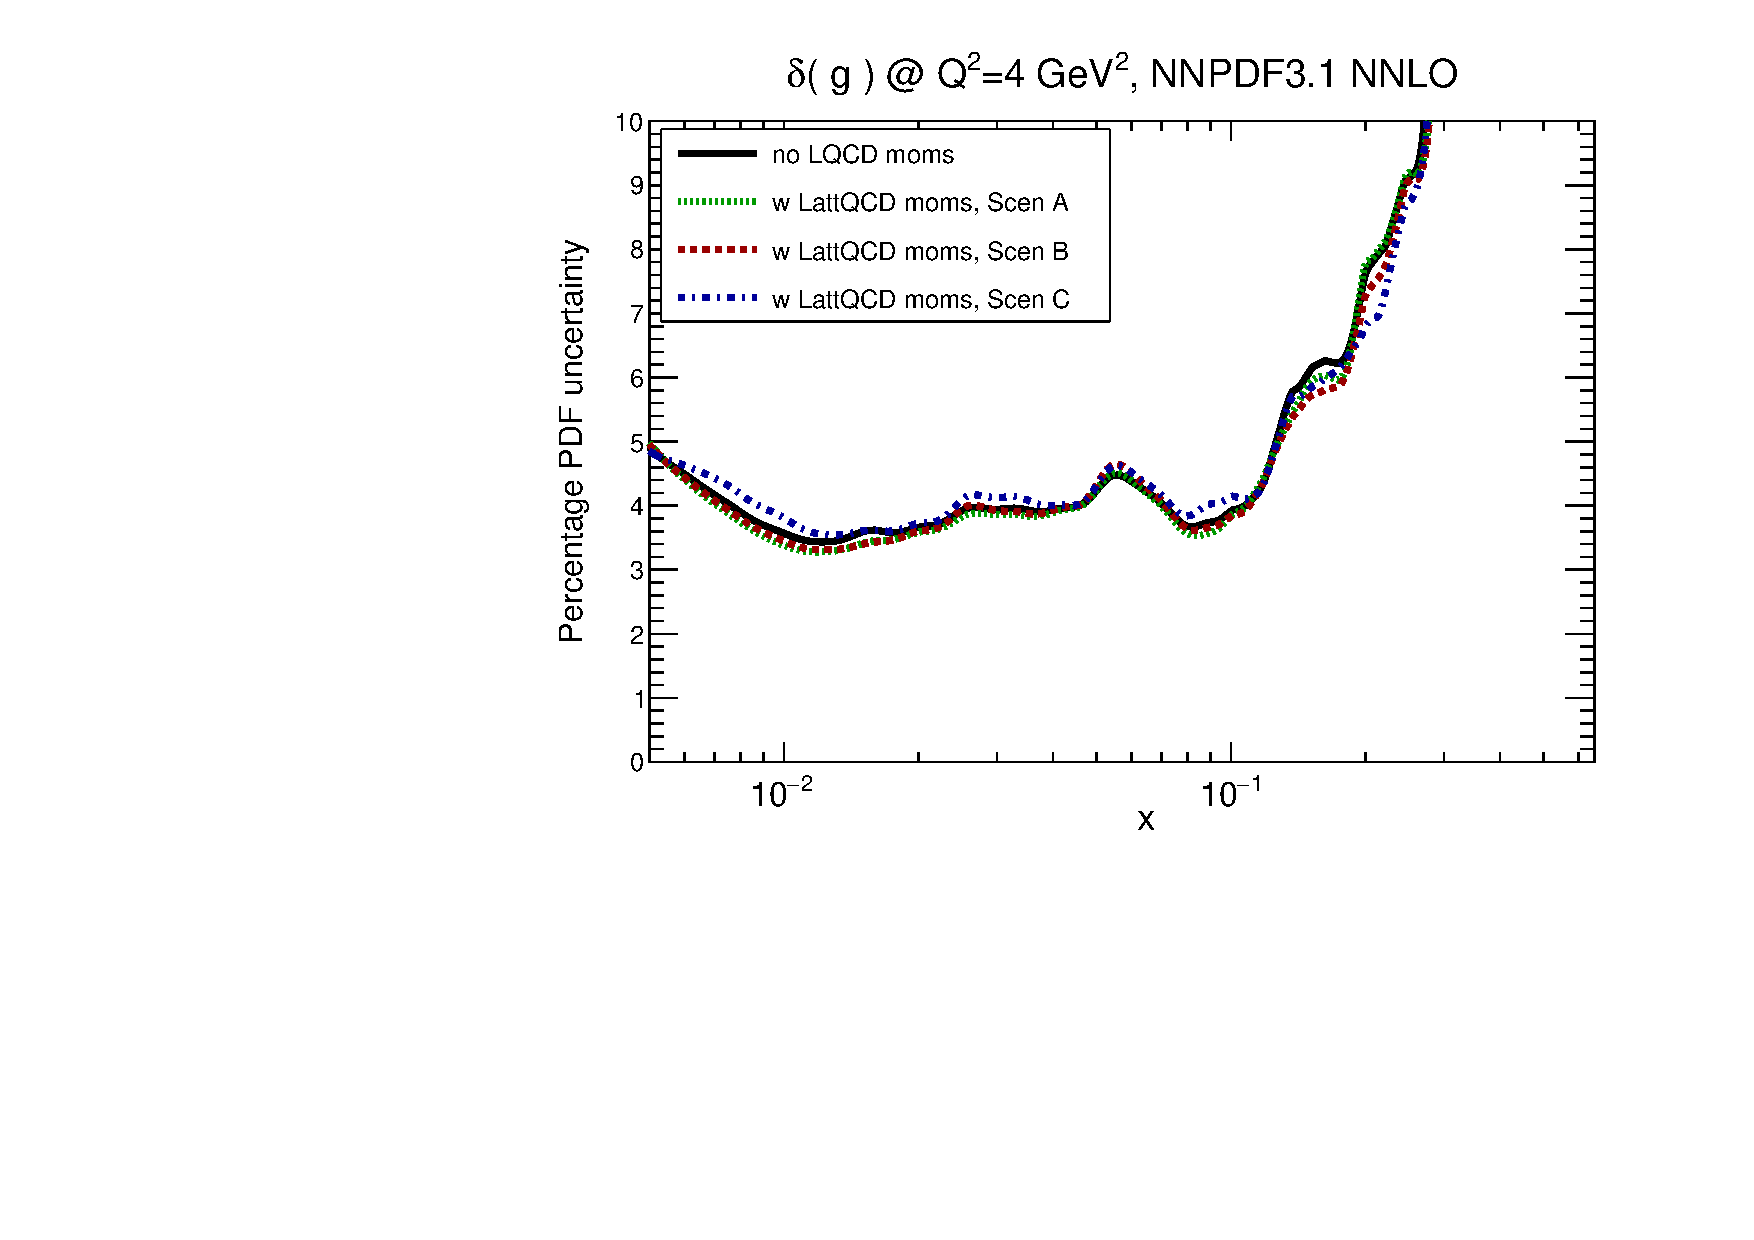
\includegraphics[scale=0.45]{plots/xg-unpol-lattice-relerr.pdf}
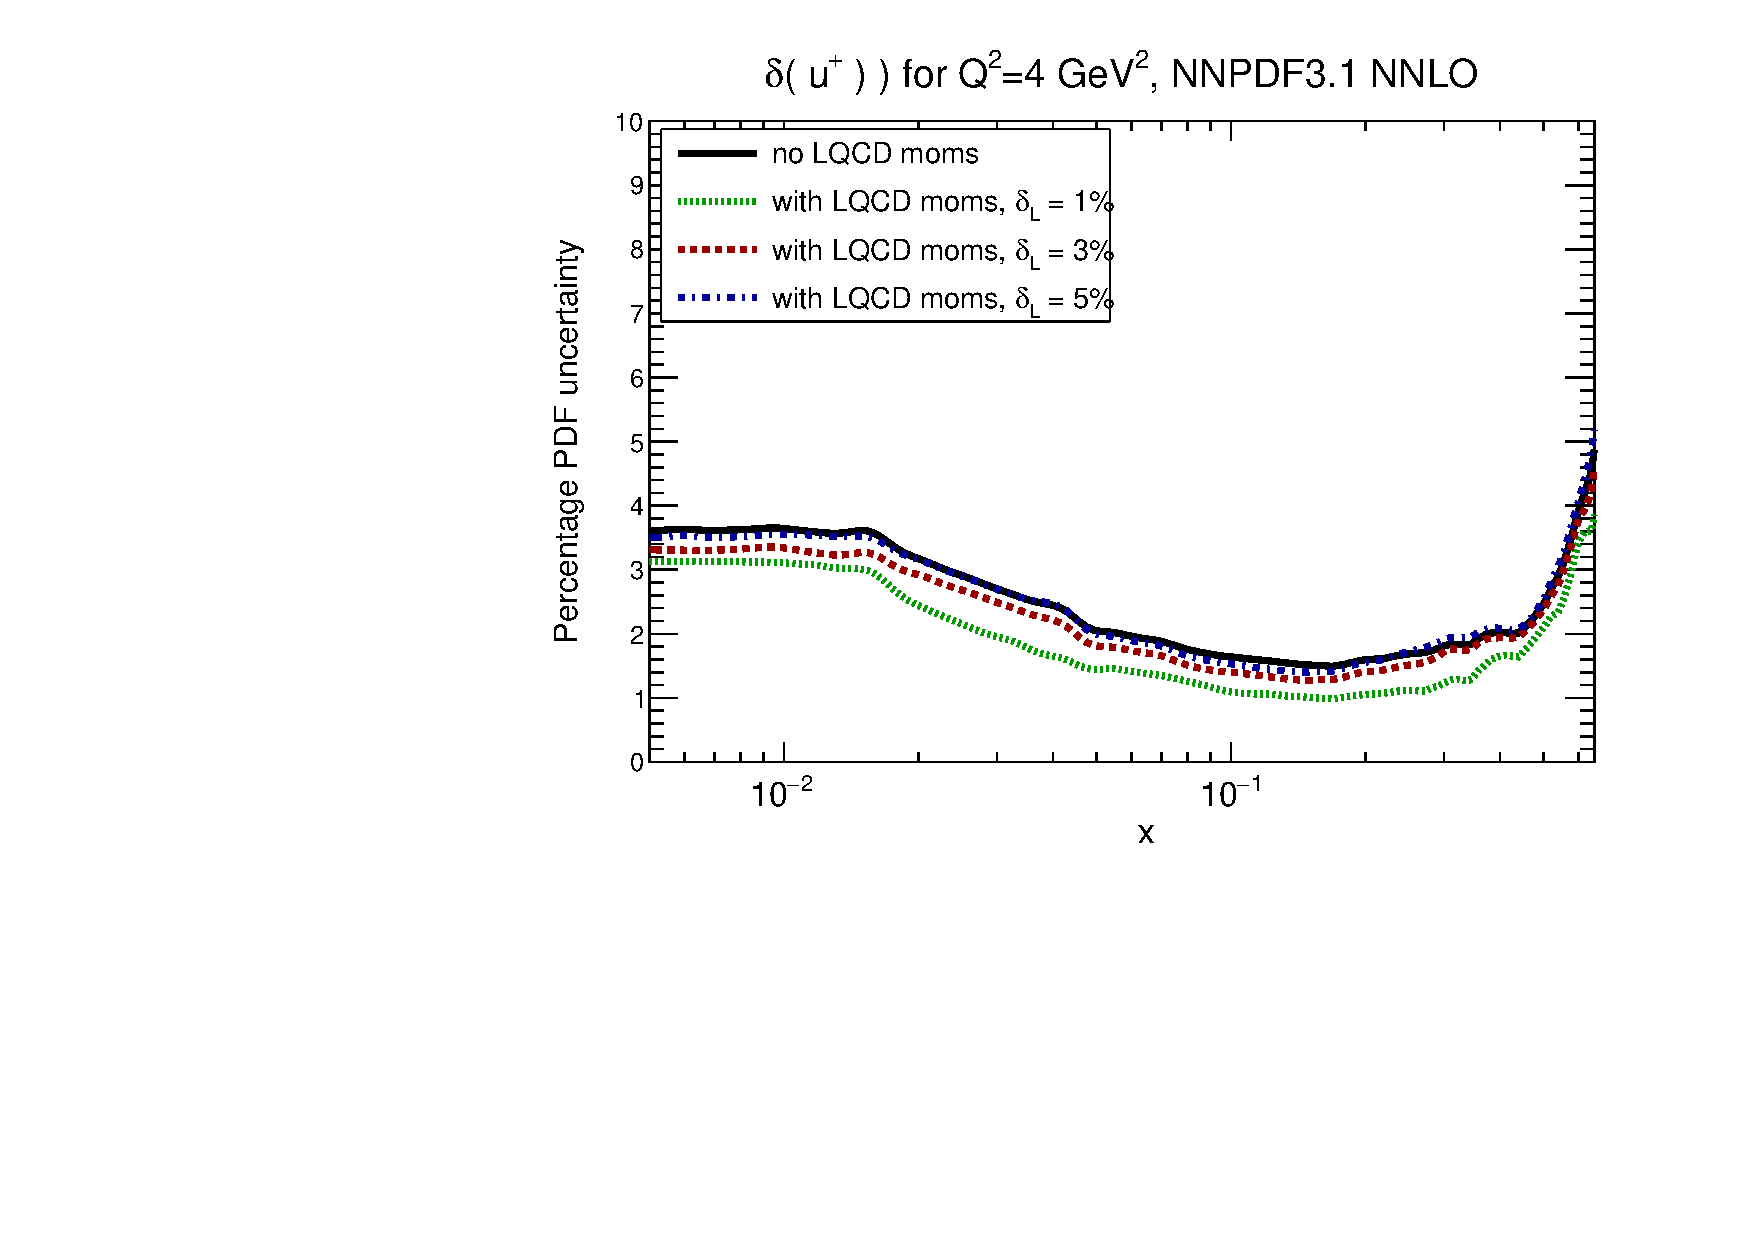
\includegraphics[scale=0.45]{plots/xup-unpol-lattice-relerr.pdf}
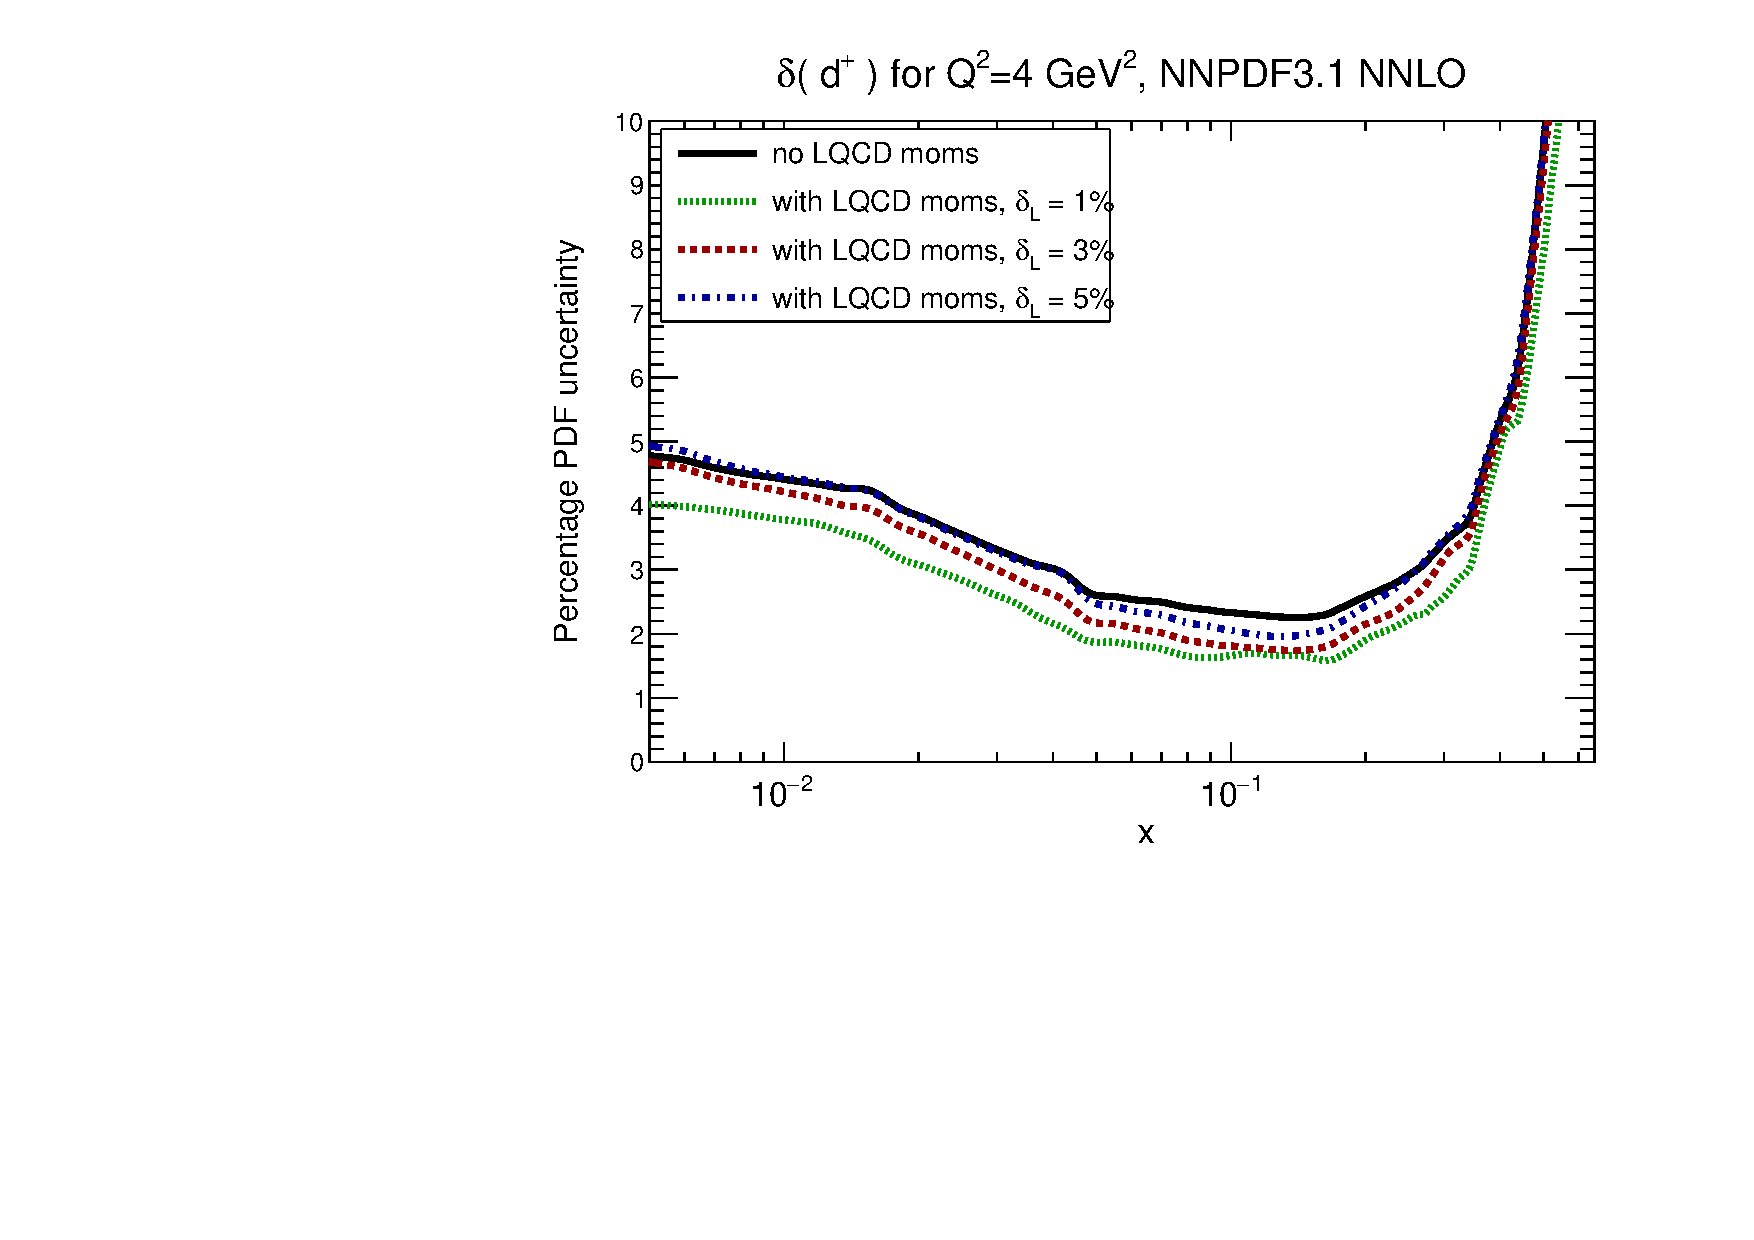
\includegraphics[scale=0.45]{plots/xdp-unpol-lattice-relerr.pdf}
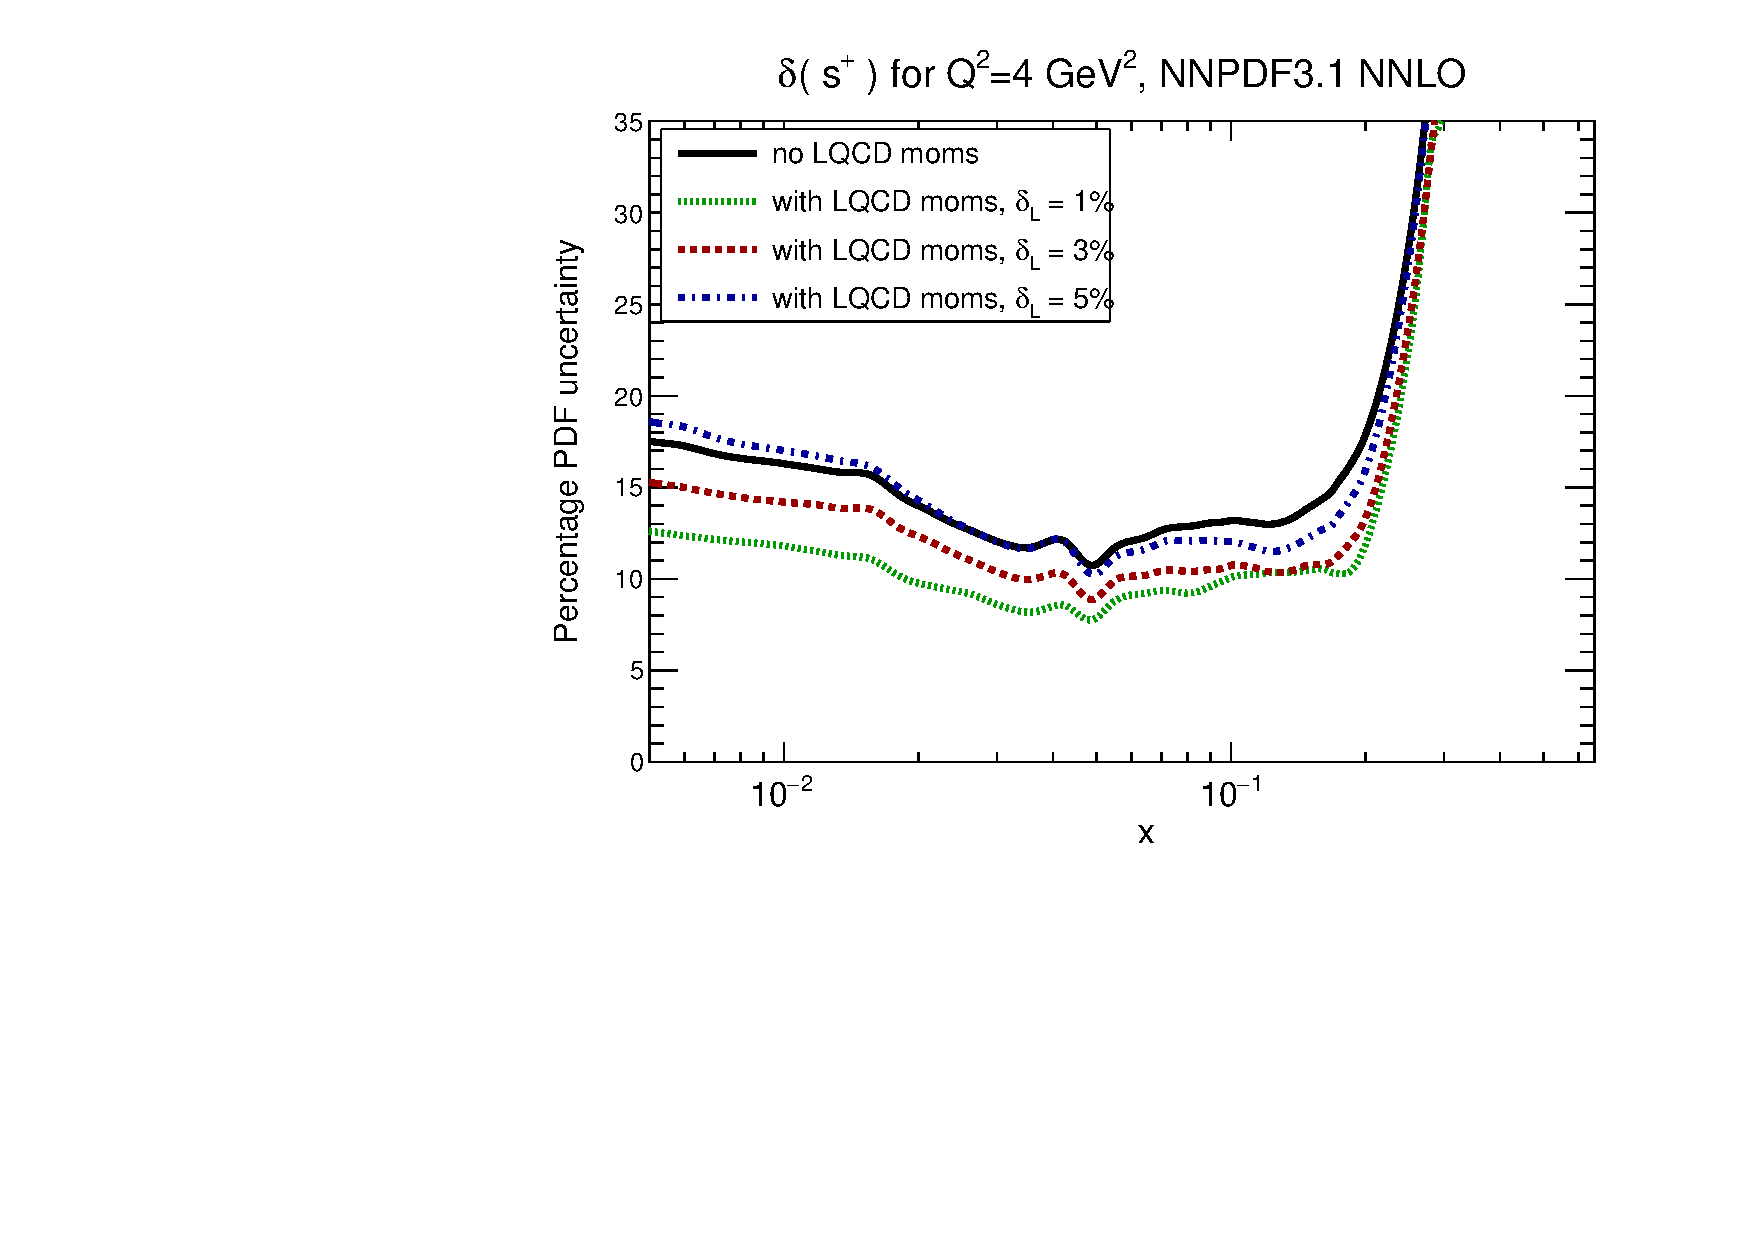
\includegraphics[scale=0.45]{plots/xsp-unpol-lattice-relerr.pdf}
\caption{\small The percentage PDF uncertainty in NNPDF3.1 NNLO
  for the gluon and the $u^+$, $d^+$ and $s^+$ quark PDFs at
  $Q^2=4$ GeV$^2$,
  compared to the results of including the five lattice
  QCD moments as pseudo-data points in the fit using the three
  different scenarios in  Table~\ref{tab:scenarios}.
  %
See text for more details.
}    
\label{fig:impactUnpol}
\end{figure}
%----------------------------------------------------------

\subsection{Impact on polarized global fits}

Next, we move to discuss the results of applying the same
reweighting procedure this time to a representative polarized
global fit, specifically NNPDFpol1.1.

First of all, in Table~\ref{tab:polmomentsrw}
we list the values of the polarized PDF moments
  used as pseudo-data, as well as the corresponding results
  after the reweighting has been performed for the
three scenarios summarized in 
in Table~\ref{tab:scenarios}.
%
The PDF uncertainties quoted correspond in all cases to 68\%
CL intervals.


%%%%%%%%%%%%%%%%%%%%%%%%%%%%%%%%%%%%%%%%%%%%%%%%%%%%%%%%
\begin{table}[h]
\centering
\begin{tabular}{c|c|c|c|c}
  \hline &  before RW  & RW Scen A  &  RW Scen B  & RW Scen C  \\
  \hline
  $\la 1\ra_{\Delta u^+}$    &  $+0.788\pm  0.079$   &  $+0.795 \pm  0.041$    &     &   \\
   $\la 1\ra_{\Delta d^+}$   &  $-0.462 \pm 0.083$  &   $-0.454\pm  0.039$  &     &   \\
  $\la 1\ra_{\Delta s^+}$    &  $-0.124\pm   0.108 $  & $ -0.115 \pm 0.021$    &     &   \\
  $\la 1\ra_{\Delta u^+ - \Delta d^+}$  & $+1.250 \pm 0.024$   & $+1.251 \pm 0.022 $    &     &   \\
  $\la x\ra_{\Delta u^--\Delta d^-}$     & $+0.196 \pm 0.014$    &  $+0.195 \pm  0.015$   &     &   \\
  \hline
\end{tabular}
\caption{\small Values of the polarized PDF moments
  used as pseudo-data, as well as the corresponding results
  after the reweighting has been performed for the
three scenarios summarized in 
in Table~\ref{tab:scenarios}.
%
The PDF uncertainties quoted correspond in all cases to 68\%
CL intervals.
\label{tab:polmomentsrw}
}
\end{table}
%%%%%%%%%%%%%%%%%%%%%%%%%%%%%%%%%%%%%%%%%%%%%%%%%%%%%%%%

In Fig.~\ref{fig:impactPol} a
similar comparison as that of Fig.~\ref{fig:impactUnpol}, now
  showing the absolute PDF uncertainties of the NNPDFpol1.1 fit
  compared to the corresponding results once the lattice pseudo-data
  on polarized moments in included in the analysis via
  reweighting.
  %
  We find that the impact of the lattice calculations
  would be more marked on the total
  strangeness PDF $\Delta s^+$.
  
%------------------------------------------------------
\begin{figure}[!t]
\centering
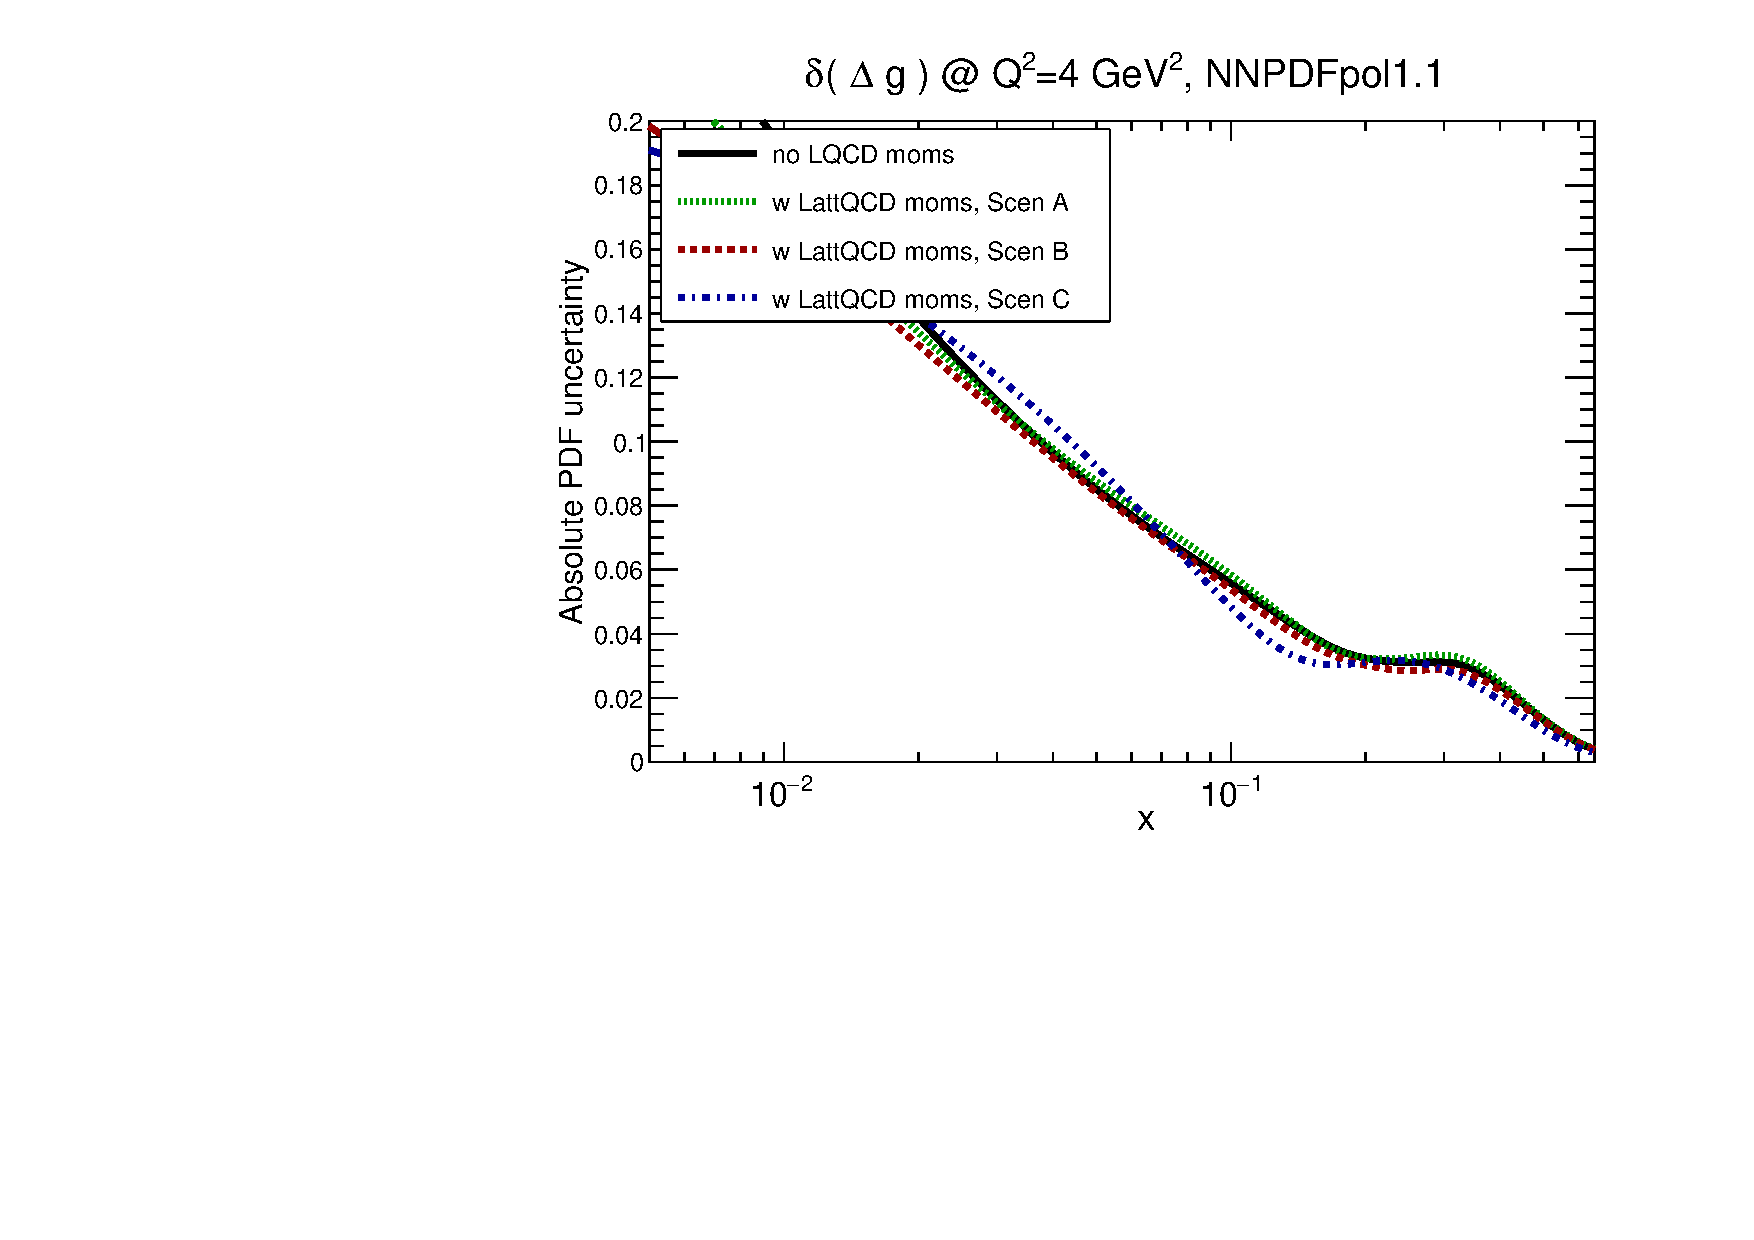
\includegraphics[scale=0.45]{plots/xg-pol-lattice-relerr.pdf}
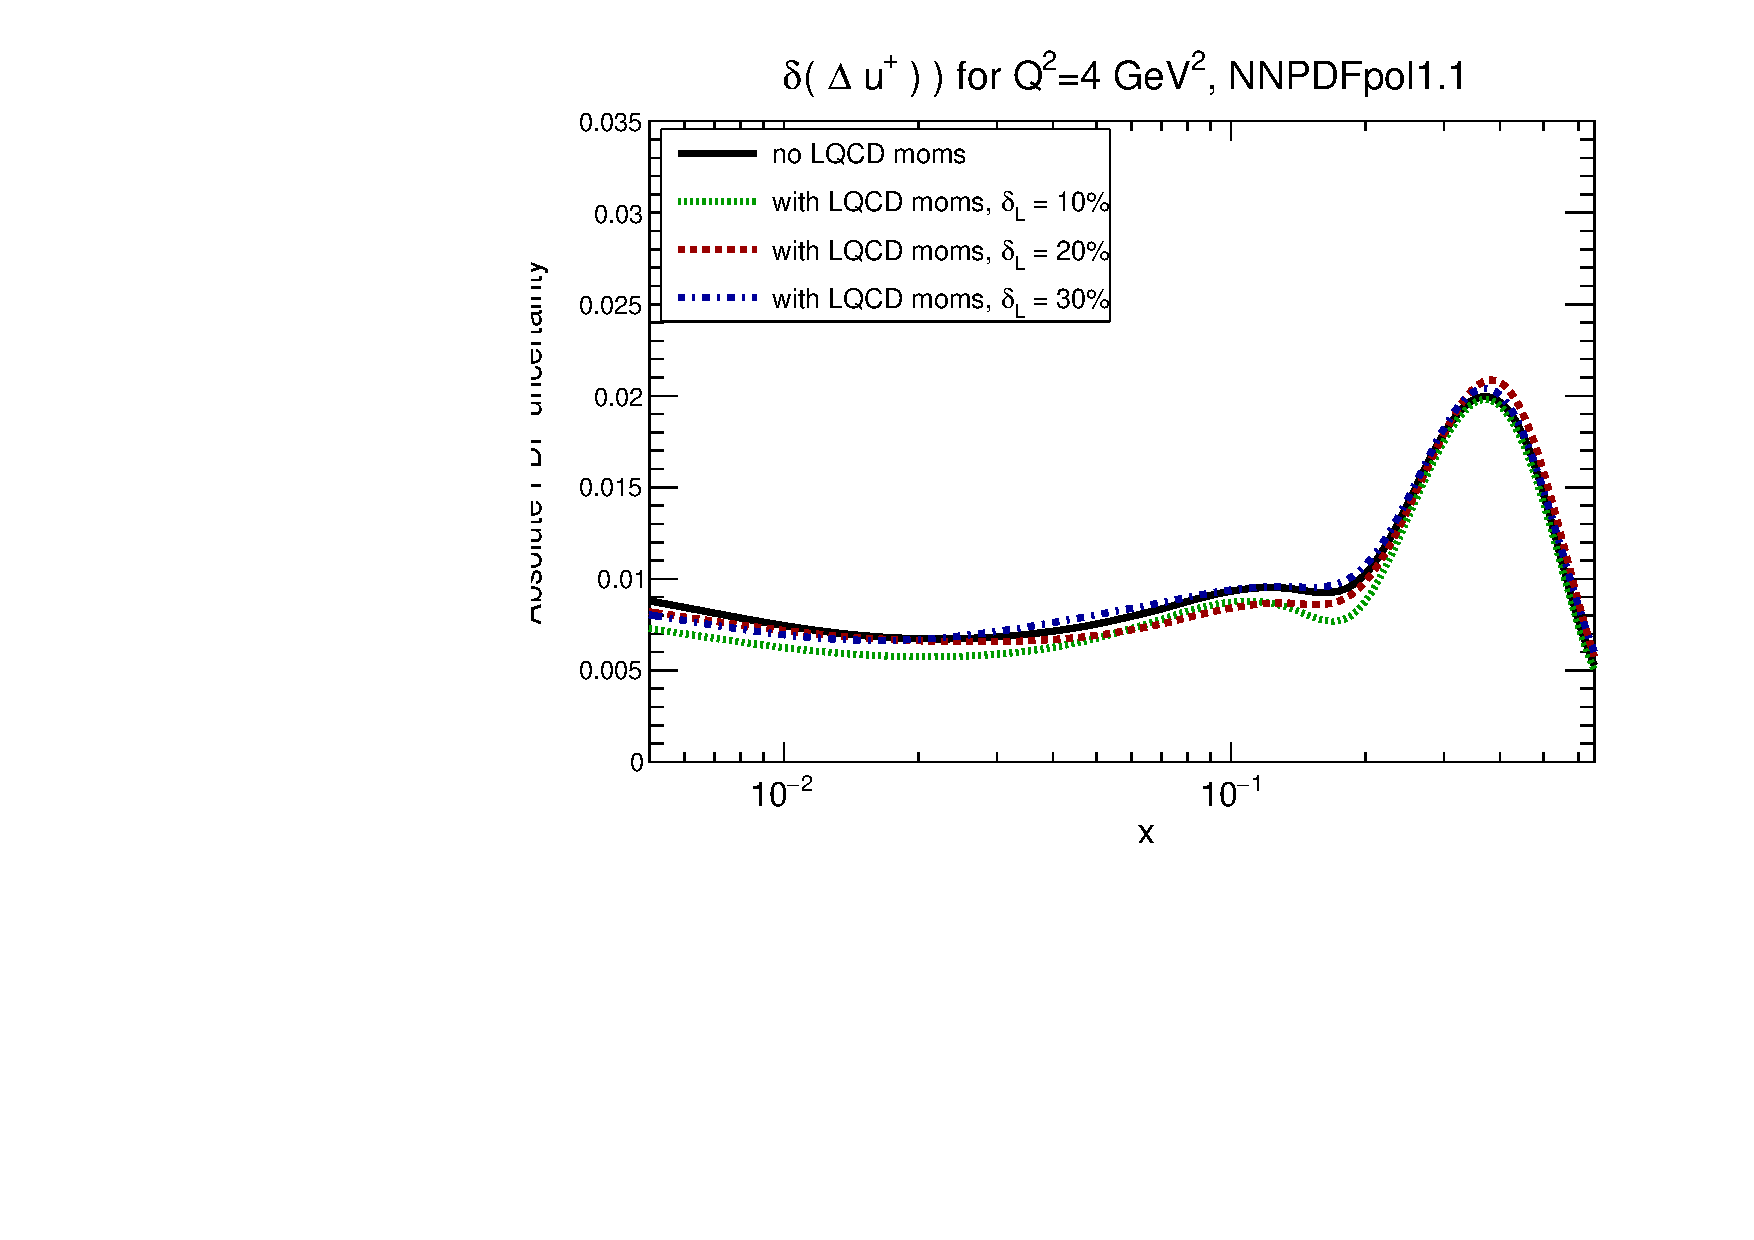
\includegraphics[scale=0.45]{plots/xup-pol-lattice-relerr.pdf}
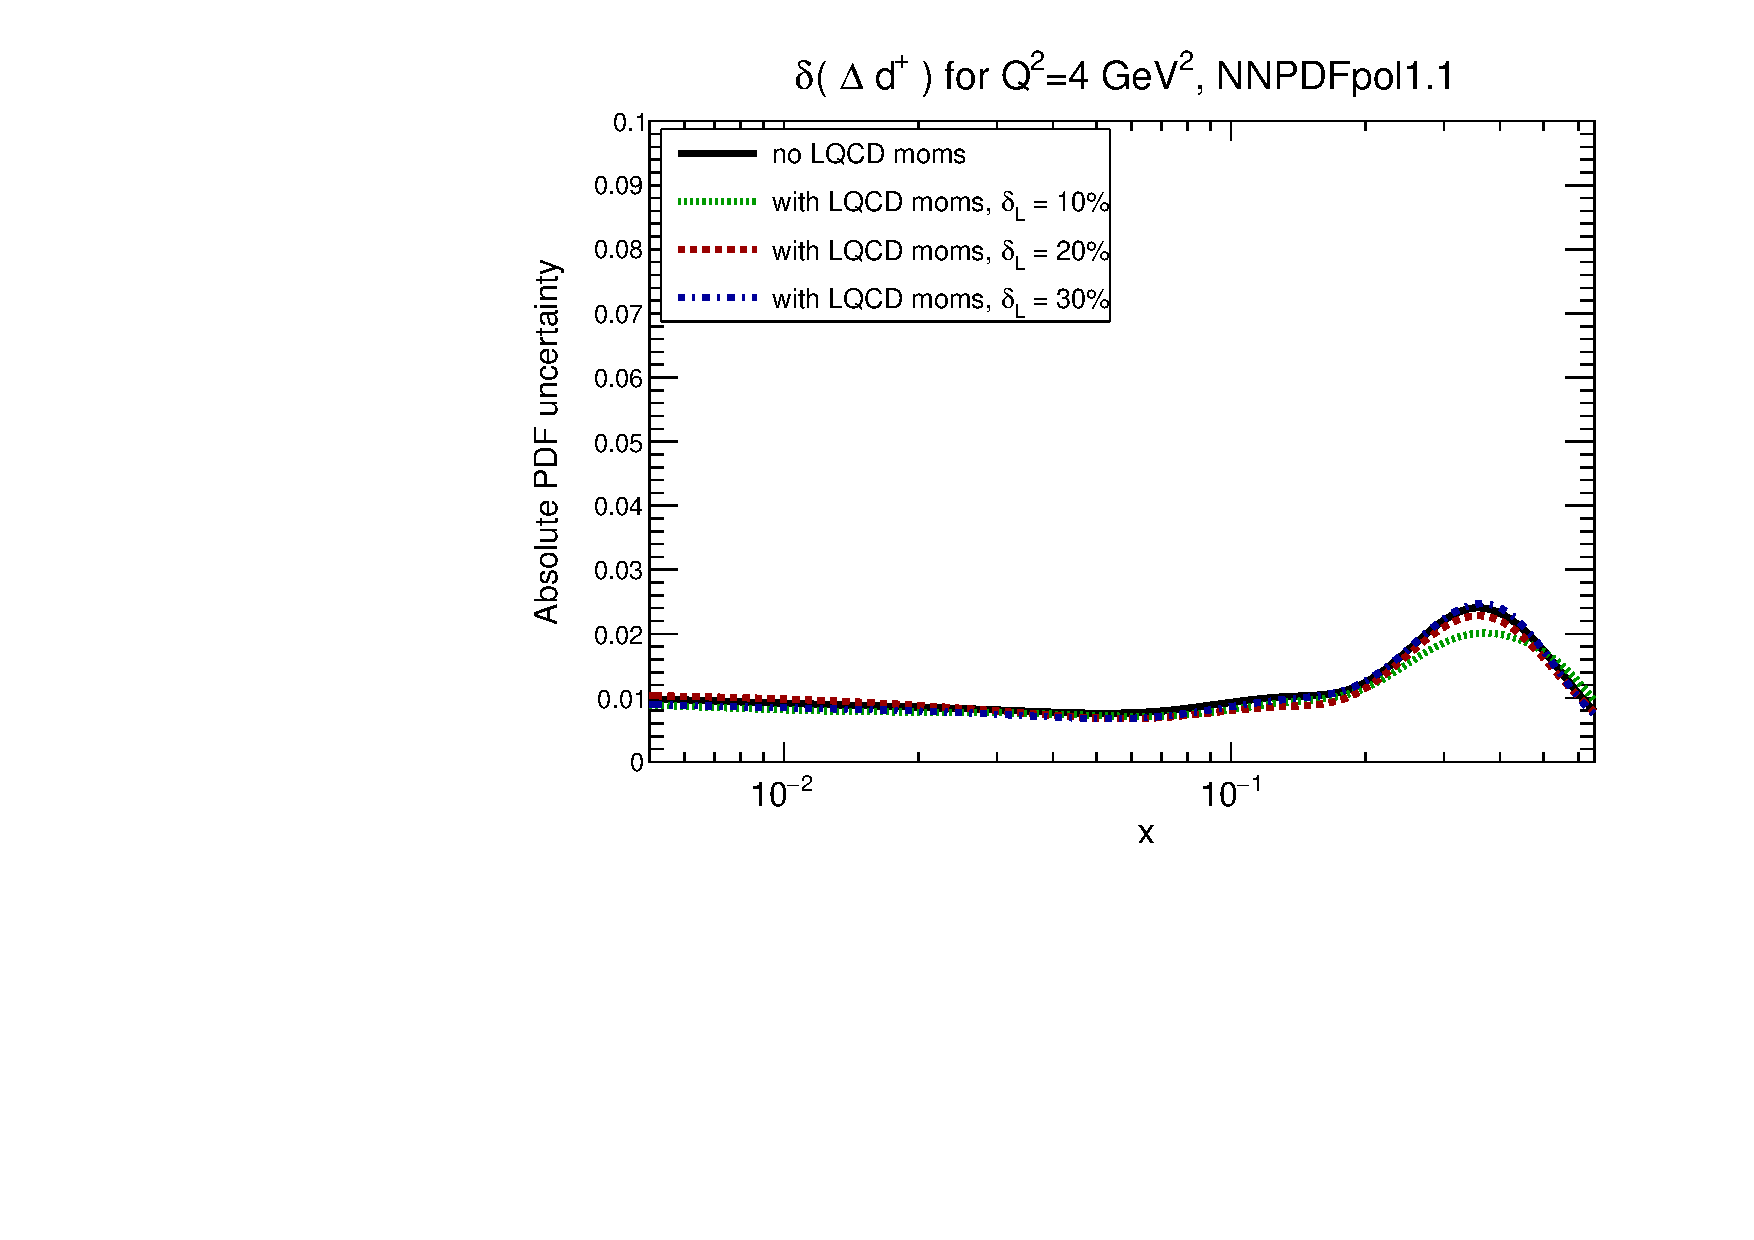
\includegraphics[scale=0.45]{plots/xdp-pol-lattice-relerr.pdf}
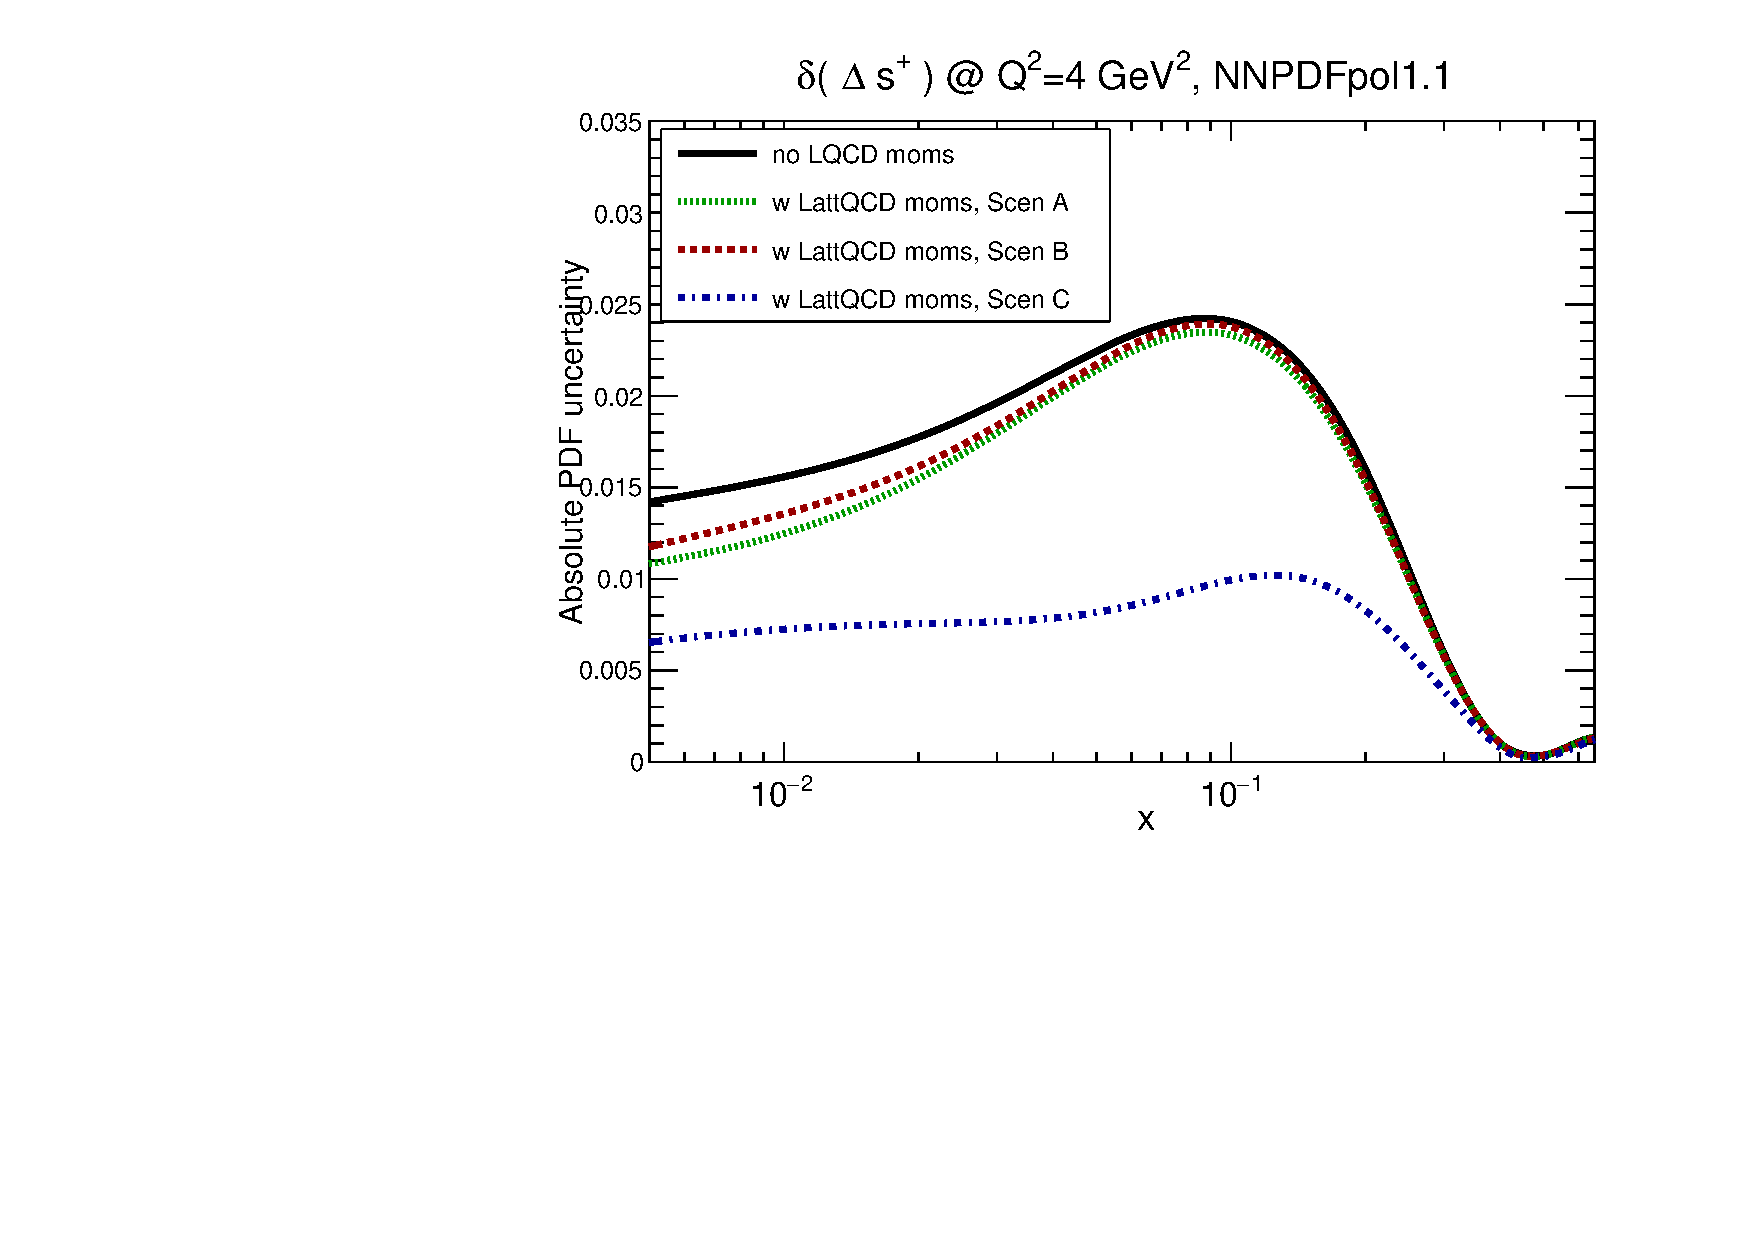
\includegraphics[scale=0.45]{plots/xsp-pol-lattice-relerr.pdf}
\caption{\small Same as Fig.~\ref{fig:impactUnpol}, now
  showing the absolute PDF uncertainties of the NNPDFpol1.1 fit
   $Q^2=4$ GeV$^2$,
  compared to the corresponding results once the lattice pseudo-data
  on polarized moments in included in the analysis via
  reweighting.
}    
\label{fig:impactPol}
\end{figure}
%----------------------------------------------------------


\clearpage
